%\catcode`~=11 % make LaTeX treat tilde (~) like a normal character
%\newcommand{\urltilde}{\kern -.15em\lower .7ex\hbox{~}\kern .04em}
%\catcode`~=13 % revert back to treating tilde (~) as an active character
%\providecommand{\abs}[1]{\left | #1\right |}

\documentclass{beamer}
\usepackage[latin1]{inputenc}
\usepackage{spverbatim}

\usetheme{default}
%Warsaw
\title[Summary of work]{Summary of work}
\author{James McMurray}
\institute{Supervisor: Nora Umbach\\Department of Psychology\\Eberhard-Karls Universit\"{a}t T\"{u}bingen}
\date{30/08/2012}
\begin{document}


\pgfdeclareimage[height=0.5cm]{logo}{exlogo.png}
\logo{\pgfuseimage{logo}}

\begin{frame}
\titlepage
\end{frame}

  \begin{frame}<beamer>
    \frametitle{Outline of talk}
    \tableofcontents
  \end{frame}


\section{TU Berlin Code}
\begin{frame}[t]{TU Berlin Code}
Provided group of testing scripts for CRT/LCD monitor, and also scripts for producing various stimuli. {\bf Calibration Tests :}
\begin{description}
\item[crttest.py] Produces a \alert{patch of a certain luminance} in the centre of the screen, and \alert{modulates the surround} according to a \alert{sin function}. On a CRT the luminance of the patch will vary, but not on an LCD. Included as {\it CRTTest()} in {\it stimuliclass.py}.\\
~\\
\item[gamma.py] Compare luminance of large patch and small patch, on a CRT, the large patch should always be less bright. Can use up and down arrow keys to modify the size of the patch whilst running. Included as {\it PatchBrightnessTest()} in {\it stimuliclass.py}
\end{description}

\end{frame}

\begin{frame}[t]{Calibration tests continued}
\begin{description}
\item[lines.py] Create series of lines, swap between horizontal and vertical - check for change in overall luminance. Included as {\it Lines()} in {\it stimuliclass.py} \\
~\\
~\\
\item[singrating.py] Produces a sin-wave based stimuli across the screen, which is then shifted to anti-phase and re-presented rapidly. Apparently should be invisible at high frequencies. Included as {\it SinGrating()} in {\it stimuliclass.py}
\end{description}

\end{frame}
\begin{frame}[t]{Stimuli}
Also provided methods to produce the following stimuli. Now implemented in {\it stimuliclass.py}.
\begin{description}
\item[Cornsweet()] Produces a form of the Cornsweet illusion to PNG if no PNG file is provided in the pngfile argument, otherwise it will display the stimuli provided.

\end{description}
\begin{figure}[c]

\includegraphics[height=3cm]{cornsweet20120814_1705.png}
\caption{The produced Cornsweet stimulus.}
\end{figure}


\end{frame}
\begin{frame}[t]{Mondrian}
\begin{description}
\item[Mondrian()] Produces a Mondrian to a PNG if no PNG file is provided in the pngfile argument, otherwise it will display the Mondrian with run(). This method is called during the generation of articulated stimuli.
\end{description}
\begin{figure}[c]
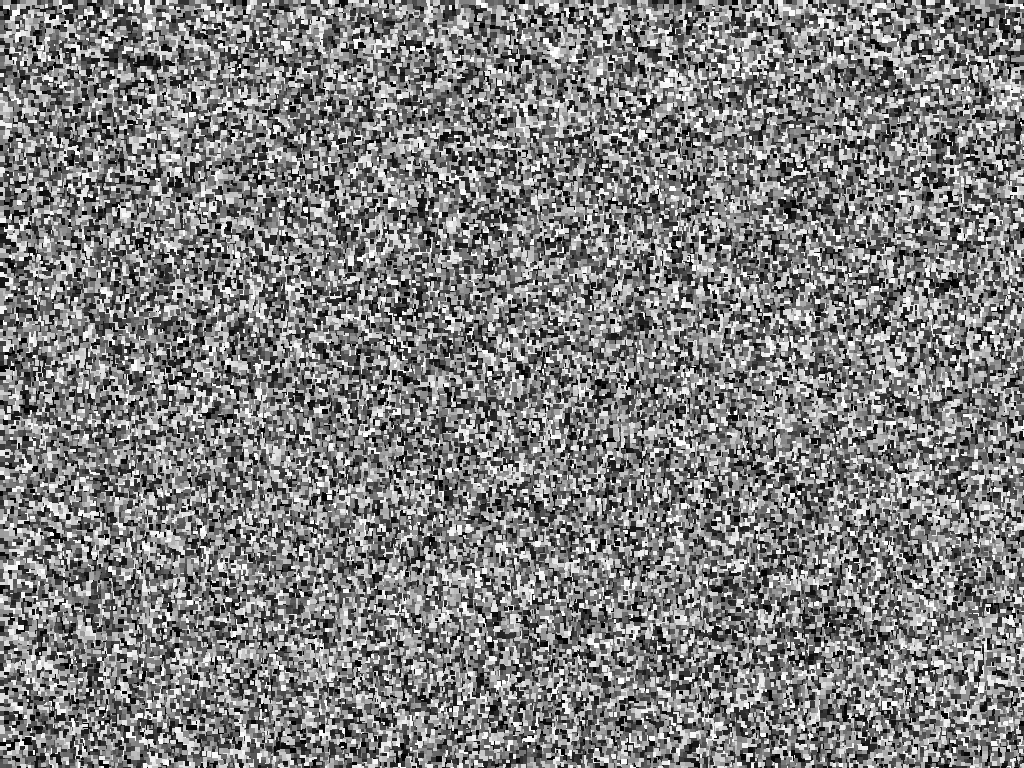
\includegraphics[height=3cm]{mondrian20120713_1126.png}
\caption{An example of a black and white Mondrian stimulus.}
\end{figure}
\end{frame}

\begin{frame}[t]{Todorovic}
\begin{description}
\item[Todorovic()] Produces a form of the Torodovic checkerboard illusion to PNG if no PNG file is provided in the pngfile argument, otherwise it will display the stimuli provided. Note that it works by first producing an appropriate Cornsweet stimulus and then repeating this.
\end{description}
\begin{figure}[c]

\includegraphics[height=3cm]{todorovic20120814_1705.png}
\caption{An example of the Todorovic stimulus.}
\end{figure}
\end{frame}

\begin{frame}[t]{White's Illusion}
\begin{description}
\item[WhiteIllusion()] Produces a form of the White's illusion on a square wave to PNG if no PNG file is provided in the pngfile argument, otherwise it will display the stimuli provided. Produces both kind=``bmcc'': in the style used by Blakeslee and McCourt (1999), and kind=``gil'': in the style used by Gilchrist (2006).
\end{description}
\begin{figure}[c]
 \centering
  \begin{minipage}[b]{5 cm}
    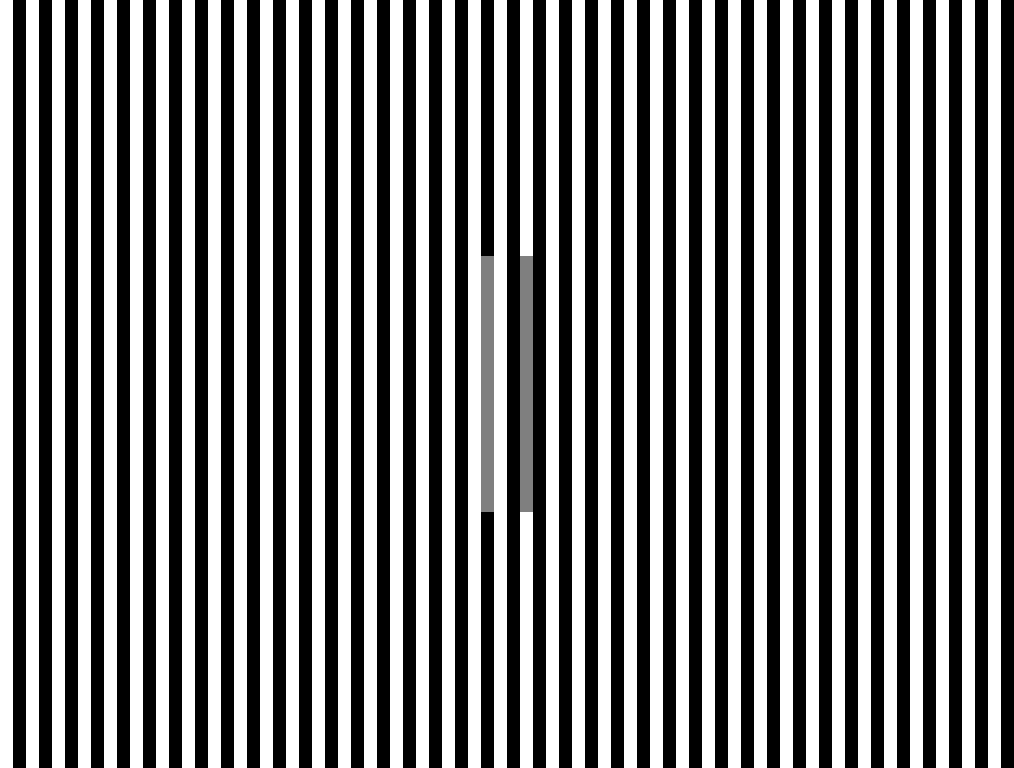
\includegraphics[height=3cm]{whiteillusionbmcc20120814_1705.png}
  \end{minipage}
  \begin{minipage}[b]{5 cm}
    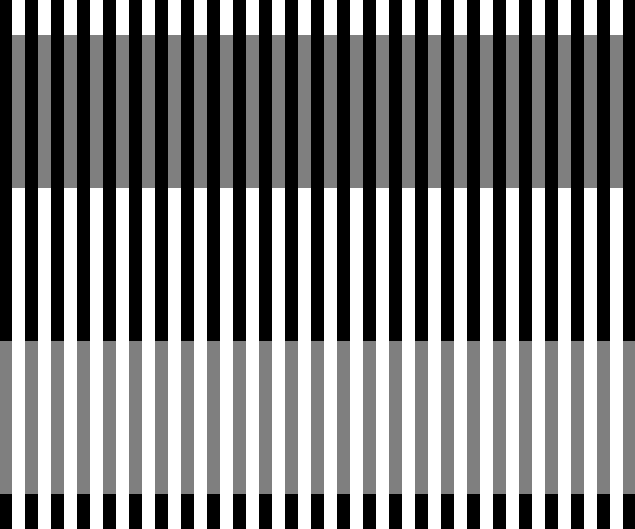
\includegraphics[height=3cm]{whiteillusiongil20120815_1138.png}
  \end{minipage}

  \caption{An example of the Blakeslee and McCourt (left) and Gilchrist (right) White's Illusion stimuli.}
\end{figure}
\end{frame}

\begin{frame}[t]{Minor issue with Stimuli generation}
~\\
Note that because some of the stimuli (Cornsweet, Todorovic, White's Illusion) usually take their arguments in \alert{visual degrees} (although it can also be provided by the \alert{pixels per degree} and \alert{monitor size}), sometimes the stimuli produced will be 1 pixel or so too large for the monitor, and so fail to display via PsychoPy.\\
~\\
I submitted a patch to PsychoPy so it now returns a warning when this happens (the monitor will just display a black screen). But it's worth remembering if dealing with these stimuli.
\end{frame}
\section{Articulated Stimuli}


\begin{frame}[t]{Articulated Stimuli}
%photo here

The stimuli are produced via the {\it articulated.py} script in {\bf achrolabutils}. 

\begin{itemize}
\item This script uses the \emph{normal distribution} to set the shades of gray, so one provides the \alert{mean} and \alert{standard deviation} of the values for both sides along with a \alert{seed} to randomise the pattern, and the \alert{mean edge length of the Mondrian rectangles}.

\item In the {\it articulated.py} script one must change the stimuli list (of infield and surround values). The script then produces all of the stimuli, matched against eachother, encoded for the Eizo monitor. Currently it produces them both with transparent infields, and with non-transparent infields.
\end{itemize}
\end{frame}

\begin{frame}[fragile]{Loading many image stimuli}
Previously the old experiment code crashed when attempting to handle so many image stimuli. This was because the code was attempting to load them \alert{all at once}, whereas the new code \alert{reloads the stimuli in to the same object} which frees the memory.\\
~\\
Don't do this:
\begin{spverbatim}
stim_0_0 =  [(0,0,0), (0,0,0), InfieldSurround(mywin, 376, 456, 376, 456, 621)]
stim_0_1 =  [(0,0,0), (0,0,0), InfieldSurround(mywin, 376, 456, 376, 456, 621)]
[...]
\end{spverbatim}
~\\
But {\bf simply replace the stimuli directly}.


\end{frame}

\section{Some problems}
\begin{frame}[t]{Some problems}
\begin{description}
\item[Re-calibration:] ~\\Re-measurement after re-calibration consistently produces different results.\\
~\\

\item[Lines stimulus:] ~\\The lines stimuli are significantly brigher when displayed horizontally, for small pixel widths ($\sim <8$).\\
~\\
\item [Tube voltage hysteresis curves:] ~\\The curves for the tube voltage against measured luminance vary depending on the direction, whether the voltage is increasing or decreasing.
\end{description}
\end{frame}

\begin{frame}[t]{Re-calibration problem}
The variance is most noticable at the higher gray values (brighter shades).

\begin{figure}[c]
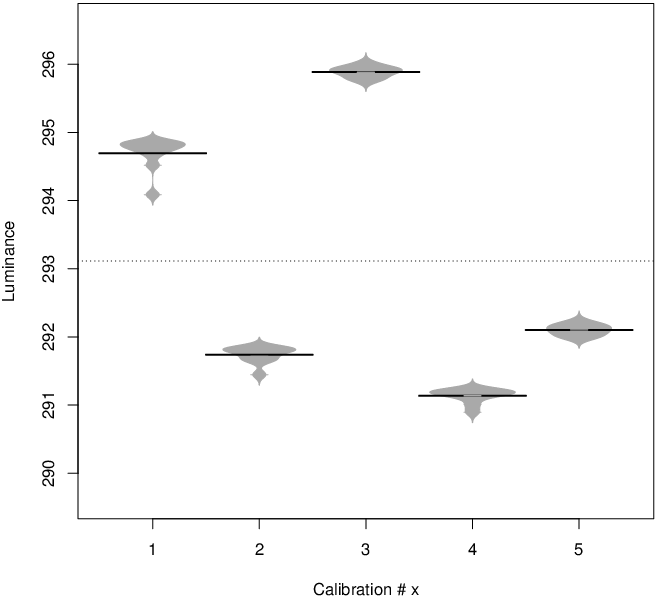
\includegraphics[height=6cm]{cbeanplotmean_800_color.png}
\caption{Bean plot showing the variance between re-calibrations at a gray value of 800.}
\end{figure}
\end{frame}

\begin{frame}[t]{Variance across gray values}
This plot shows the variance across gray values.
\begin{figure}[c]
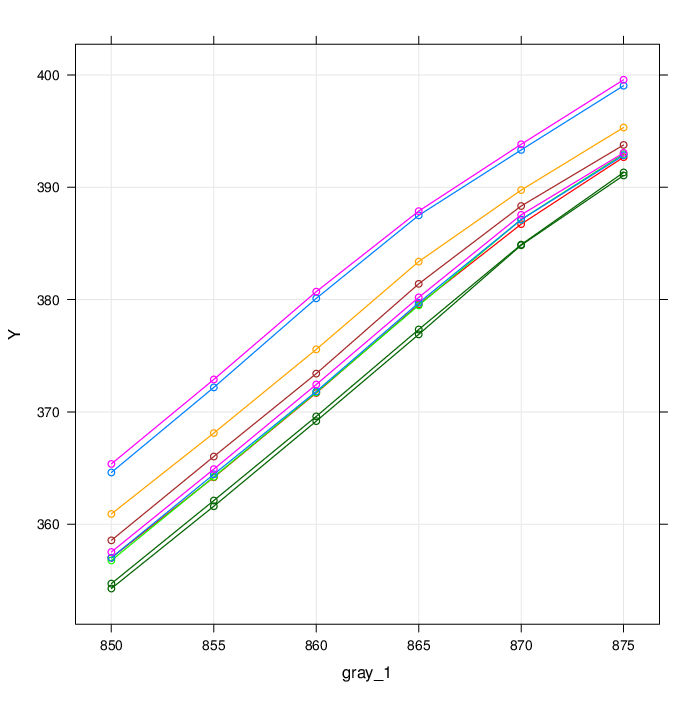
\includegraphics[height=8cm]{highend.png}
\end{figure}
\end{frame}
%Problems - calibration beanplots, lines problem



\begin{frame}[t]{Lines luminance difference}
This is a plot of the luminance for 1-pixel wide lines measured at the observer distance. The red line is for vertical lines, and the black for horizontal. The effect is visible by eye.
\begin{figure}[c]
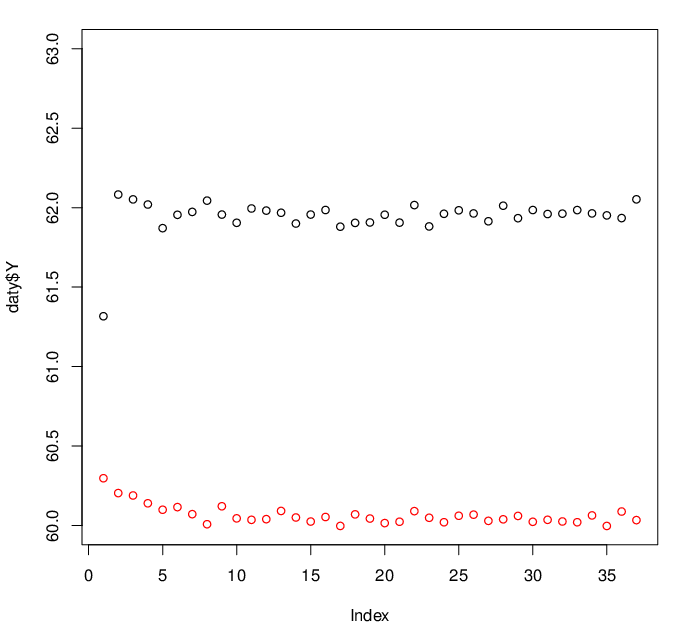
\includegraphics[height=7cm]{line1dist.png}
\end{figure}
\end{frame}

\begin{frame}[t]{Lines luminance difference}
This is a plot of the luminance for 8-pixel wide lines measured at the observer distance. The red line is for vertical lines, and the black for horizontal. The difference becomes negligible.
\begin{figure}[c]
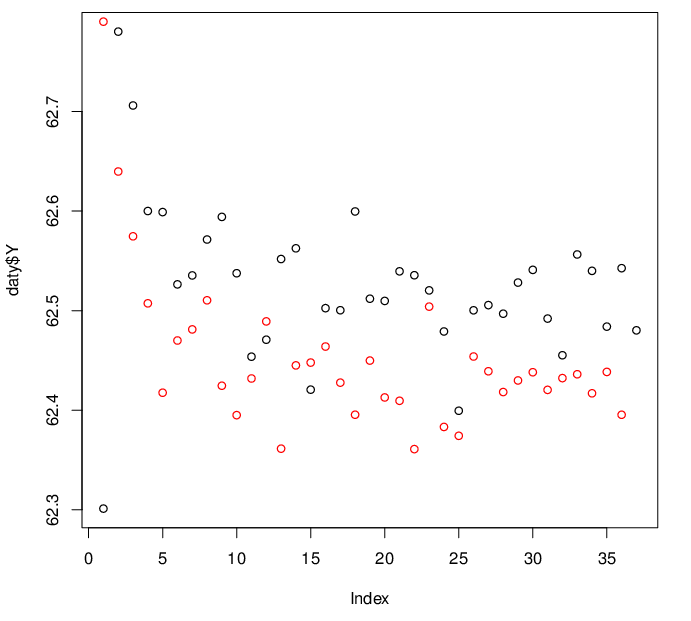
\includegraphics[height=7cm]{line8dist.png}
\end{figure}
\end{frame}

\begin{frame}[t]{Tube voltage hysteresis curves}
This is a plot of luminance against tube voltage for the green tube. The black line is for decreasing voltage, and the green line for increasing voltage. Evidently, they don't match.
\begin{figure}[c]
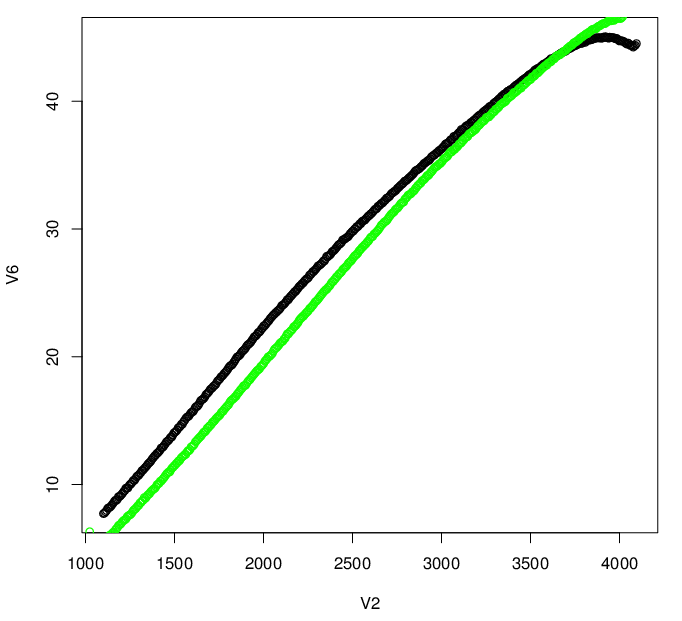
\includegraphics[height=7cm]{greenhysteresis.png}
\end{figure}
\end{frame}


\section{Results}
\begin{frame}[t]{Results from articulated stimuli experiment}
Results here
\end{frame}

\begin{frame}[t]{Tube voltage hysteresis curves}
This is a plot of luminance against tube voltage for the red tube. The black line is for decreasing voltage, and the red line for increasing voltage. Evidently, they don't match.
\begin{figure}[c]
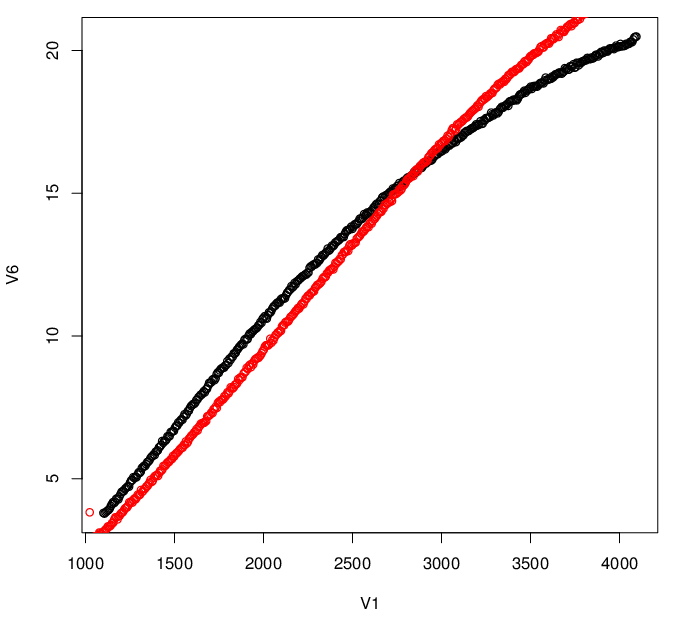
\includegraphics[height=7cm]{redhysteresis.png}
\end{figure}
\end{frame}

\begin{frame}[t]{Tube voltage hysteresis curves}
This is a plot of luminance against tube voltage for the blue tube. The black line is for decreasing voltage, and the blue line for increasing voltage. Evidently, they don't match.
\begin{figure}[c]
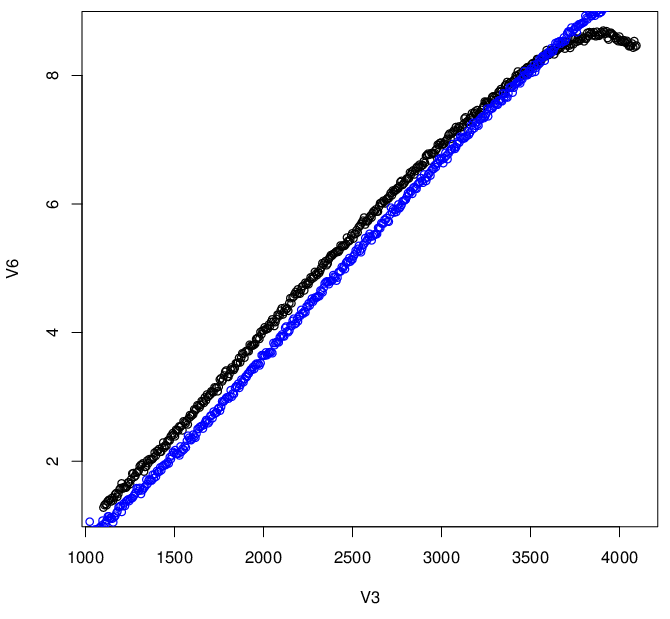
\includegraphics[height=7cm]{bluehysteresis.png}
\end{figure}
\end{frame}

\begin{frame}[t]{Tube voltage hysteresis curves}
This is a plot of luminance against tube voltage for all tube. The black line is for decreasing voltage, and the blue line for increasing voltage. Evidently, they don't match.
\begin{figure}[c]
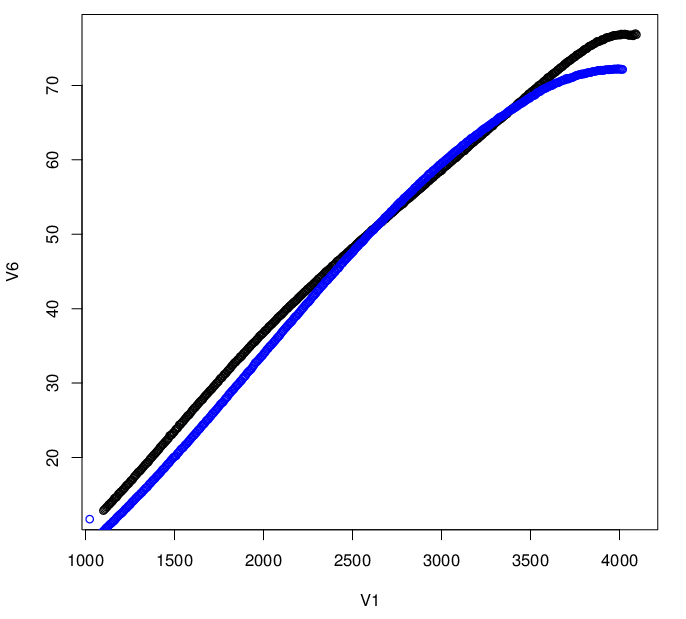
\includegraphics[height=7cm]{allhysteresis.png}
\end{figure}
\end{frame}

\end{document}
